% Created 2021-11-23 Tue 09:03
% Intended LaTeX compiler: pdflatex
\documentclass[presentation,aspectratio=1610]{beamer}
\usepackage[utf8]{inputenc}
\usepackage[T1]{fontenc}
\usepackage{graphicx}
\usepackage{grffile}
\usepackage{longtable}
\usepackage{wrapfig}
\usepackage{rotating}
\usepackage[normalem]{ulem}
\usepackage{amsmath}
\usepackage{textcomp}
\usepackage{amssymb}
\usepackage{capt-of}
\usepackage{hyperref}
\usepackage{khpreamble, euscript}
\DeclareMathOperator{\atantwo}{atan2}
\newcommand*{\ctrb}{\EuScript{C}}
\newcommand*{\obsv}{\EuScript{O}}
\usetheme{default}
\author{Kjartan Halvorsen}
\date{\today}
\title{Discrete-time State feedback}
\hypersetup{
 pdfauthor={Kjartan Halvorsen},
 pdftitle={Discrete-time State feedback},
 pdfkeywords={},
 pdfsubject={},
 pdfcreator={Emacs 26.3 (Org mode 9.4.6)}, 
 pdflang={English}}
\begin{document}

\maketitle

\section{Discret-time state space model}
\label{sec:org94bda5c}
\begin{frame}[label={sec:org2a875e6}]{The discrete-time state-space model}
\end{frame}

\begin{frame}[label={sec:orgd0007cb}]{The discrete-time state-space model}
\begin{center}
  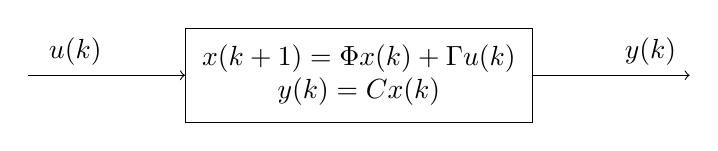
\begin{tikzpicture}[node distance=42mm, block/.style={inner sep=6pt, rectangle, draw, minimum width=15mm}, sumnode/.style={circle, draw, inner sep=2pt}]
    \node[coordinate] (input) {};
    \node[block, right of=input, align=center] (plant)  {$x(k+1) = \Phi x(k) + \Gamma u(k)$\\$y(k) = C x(k)$};
    \node[coordinate, right of=plant] (output) {};

    \draw[->] (input) -- node[above, pos=0.3] {$u(k)$} (plant);
    \draw[->] (plant) -- node[above, near end] {$y(k)$} (output);
  \end{tikzpicture}
\end{center}
\end{frame}


\section{PMSM - sysid}
\label{sec:org8f4c529}

\begin{frame}[label={sec:org4fc96f8}]{Obtain state-space model from discrete-time pulse-transfer function}
\end{frame}

\begin{frame}[label={sec:orgb5bf028}]{The permanent magnet synchronous motor}
\begin{center}
\includegraphics[width=0.9\linewidth]{../../figures/permanent-motor.jpg}
\end{center}
\end{frame}

\begin{frame}[label={sec:orgb21b305}]{The PMSM}
\begin{center}
\includegraphics[width=0.8\linewidth]{../../figures/pmsm_control_block_diag.png}
\end{center}
{\footnotesize Liu and Li  ``Speed control for PMSM servo system'', IEEE Transactions on Industrial Electronics, 2012.}
\end{frame}
\begin{frame}[label={sec:org4b44d9c}]{Identified model}
Two poles, two zeros, one delay
\begin{center}
  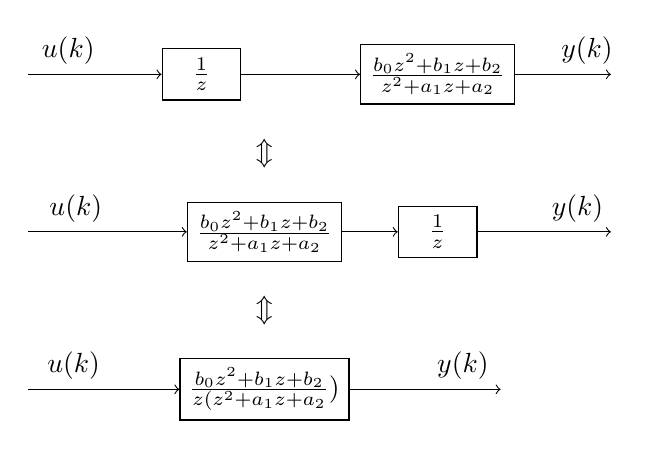
\begin{tikzpicture}[node distance=22mm, block/.style={rectangle, draw, minimum width=10mm}, sumnode/.style={circle, draw, inner sep=2pt}]

    \node[coordinate] (input) {};
    \node[block, right of=input] (delay1)  {$\frac{1}{z}$};
    \node[block, right of=delay1, node distance=30mm] (plant)  {$\frac{b_0z^2 + b_1z + b_2}{z^2 + a_1 z + a_2}$};
    \node[coordinate, right of=plant] (output) {};

    \draw[->] (input) -- node[above, pos=0.3] {$u(k)$} (delay1);
    \draw[->] (delay1) -- node[above, pos=0.3] {} (plant);
    \draw[->] (plant) -- node[above, near end] {$y(k)$} (output);

    \begin{scope}[yshift=-1cm, xshift = 3cm]
    \node {$\Updownarrow$};
    \end{scope}
    \begin{scope}[yshift=-3cm, xshift = 3cm]
    \node {$\Updownarrow$};
    \end{scope}

    \node[coordinate, below of=input, node distance=2cm] (input2) {};
    \node[block, right of=input2, node distance=30mm] (plant)  {$\frac{b_0z^2 + b_1z + b_2}{z^2 + a_1 z + a_2}$};
    \node[block, right of=plant] (delay2)  {$\frac{1}{z}$};
    \node[coordinate, right of=delay2] (output) {};

    \draw[->] (input2) -- node[above, pos=0.3] {$u(k)$} (plant);
    \draw[->] (plant) -- node[above, pos=0.3] {} (delay2);
    \draw[->] (delay2) -- node[above, near end] {$y(k)$} (output);

    \node[coordinate, below of=input2, node distance=2cm] (input3) {};
    \node[block, right of=input3, node distance=30mm] (plant)  {$\frac{b_0z^2 + b_1z + b_2}{z(z^2 + a_1 z + a_2})$};
    \node[coordinate, right of=plant, node distance=30mm] (output) {};

    \draw[->] (input3) -- node[above, pos=0.3] {$u(k)$} (plant);
    \draw[->] (plant) -- node[above, near end] {$y(k)$} (output);



  \end{tikzpicture}
\end{center}
\end{frame}

\begin{frame}[label={sec:org50003c7}]{Identified model}
\[ H(z) = \frac{6.91z^2 + 16.48z -17.87}{z(z^2 - 1.766z + 0.7665)} = \frac{6.91(z+3.19)(z-0.81)}{z(z-0.998)(z-0.768)}\]
\end{frame}

\begin{frame}[label={sec:orge0a0d61}]{From pulse-transfer function to state space model}
\begin{center}
  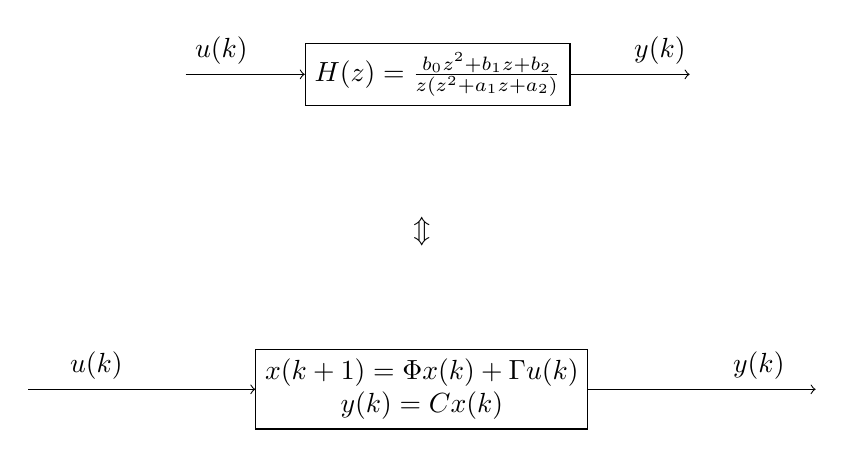
\begin{tikzpicture}[node distance=32mm, block/.style={rectangle, draw, minimum width=15mm}, sumnode/.style={circle, draw, inner sep=2pt}]

    \node[coordinate] (input) {};
    \node[block, right of=input] (plant)  {$H(z) = \frac{b_0z^2 + b_1z + b_2}{z(z^2 + a_1 z + a_2)}$};
    \node[coordinate, right of=plant] (output) {};

    \draw[->] (input) -- node[above, pos=0.3] {$u(k)$} (plant);
    \draw[->] (plant) -- node[above, near end] {$y(k)$} (output);

    \begin{scope}[yshift=-2cm, xshift = 3cm]
    \node {$\Updownarrow$};
    \end{scope}

    \begin{scope}[yshift=-4cm, node distance=50mm, xshift=-2cm]
    \node[coordinate] (input) {};
    \node[block, right of=input, align=center] (plant)  {$x(k+1) = \Phi x(k) + \Gamma u(k)$\\$y(k) = C x(k)$};
    \node[coordinate, right of=plant] (output) {};

    \draw[->] (input) -- node[above, pos=0.3] {$u(k)$} (plant);
    \draw[->] (plant) -- node[above, near end] {$y(k)$} (output);
    \end{scope}



  \end{tikzpicture}
\end{center}
\end{frame}

\begin{frame}[label={sec:org82965d6}]{Canonical forms}
Given pulse-transfer function 
\[ H(z) = \frac{b_1 z^2 + b_2 z + b_3}{z^3 + a_1z^2 + a_2z + a_3}.\] 
Find a representation in state space form
\begin{align*}
 x(k+1) &= \Phi x(k) + \Gamma u(k) \\
 y(k) &= C x(k)
 \end{align*}

\pause

\begin{itemize}
\item Controlable canonical form
\item Observable canonical form
\end{itemize}
\end{frame}

\begin{frame}[label={sec:org11e0a2a}]{Controllable canonical form}
Given pulse-transfer function 
\[ H(z) = \frac{b_1 z^2 + b_2 z + b_3}{z^3 + a_1z^2 + a_2z + a_3}.\] 

\begin{align*}
 x(k+1) &= \begin{bmatrix} -a_1 & -a_2 & -a_3\\1 & 0 & 0\\0 & 1 & 0\end{bmatrix} x(k) + \begin{bmatrix}1\\0\\0\end{bmatrix} u(k) \\
 y(k) &= \begin{bmatrix} b_1 & b_2 & b_3 \end{bmatrix} x(k)
 \end{align*}
\end{frame}


\begin{frame}[label={sec:orgc102ae9}]{Observable canonical form}
Given pulse-transfer function 
\[ H(z) = \frac{b_1 z^2 + b_2 z + b_3}{z^3 + a_1z^2 + a_2z + a_3}.\] 

\begin{align*}
 x(k+1) &= \begin{bmatrix} -a_1 & 1 & 0\\-a_2 & 0 & 1\\-a_3 & 0 & 0\end{bmatrix} x(k) + \begin{bmatrix}b_1\\b_2\\b_3\end{bmatrix} u(k) \\
 y(k) &= \begin{bmatrix} 1 & 0 & 0 \end{bmatrix} x(k)
 \end{align*}
\end{frame}


\begin{frame}[label={sec:org29c6710}]{Canonical forms}
\alert{Activity} Find the controllable canonical form for the pulse-transfer function of the motor (needed for question 2 on the exercises).

\[ H(z) = \frac{6.91z^2 + 16.48z -17.87}{z(z^2 - 1.766z + 0.7665)} = \frac{6.91(z+3.19)(z-0.81)}{z(z-0.998)(z-0.768)}\]

\pause

\begin{center}
  \includegraphics[width=.6\linewidth]{../../figures/discrete-controllable.png}
\end{center}
\end{frame}

\section{Apollo moon lander}
\label{sec:org5cca4ce}
\begin{frame}[label={sec:org9930f8c}]{Discretizing a continuous-time state-space model}
\end{frame}

\begin{frame}[label={sec:orgd570eaa}]{Example - The Apollo lunar module}
\begin{center}
\includegraphics[width=\linewidth]{../../figures/fig-apollo}
\end{center}
\end{frame}

\begin{frame}[label={sec:orgd51ff9a}]{Example - The Apollo lunar module}
State variables: \(x = \begin{bmatrix} x_1 & x_2 & x_3 \end{bmatrix}^T = \begin{bmatrix} \dot{\theta} & \theta & \dot{z} \end{bmatrix}^T\). With dynamics
\[ \begin{cases} \dot{x}_1 =  \ddot{\theta} = \frac{1}{J} u\\ \dot{x}_2 = \dot{\theta} = x_1\\ \dot{x}_3 = \ddot{z} = g\theta = gx_2 \end{cases} \]

\[ \dot{x} = \begin{bmatrix} \dot{x}_1\\\dot{x}_2\\\dot{x}_3\end{bmatrix} = \underbrace{\begin{bmatrix} \textcolor{red!60!black}{0} & \textcolor{red!60!black}{0} &\textcolor{red!60!black}{0} \\\textcolor{red!60!black}{1} & \textcolor{red!60!black}{0}& \textcolor{red!60!black}{0}\\ \textcolor{red!60!black}{0}& \textcolor{red!60!black}{g} &\textcolor{red!60!black}{0} \end{bmatrix}}_{A} \begin{bmatrix} x_1\\x_2\\x_3\end{bmatrix} + \underbrace{\begin{bmatrix} \textcolor{red!60!black}{\frac{1}{J}} \\ \textcolor{red!60!black}{0} \\\textcolor{red!60!black}{0}  \end{bmatrix}}_{B} u \]
\end{frame}

\section{Discretization}
\label{sec:org1f5260c}

\begin{frame}[label={sec:org818e46f}]{Discretization}
The general solution to a linear, continuous-time state-space system
\begin{align*}
x(t_k+\tau)& = \mathrm{e}^{A(\tau)} x(t_k) + \int_{0}^\tau \mathrm{e}^{As} B u\big((t_k+\tau)-s) ds
\end{align*}

\pause

\begin{center}
  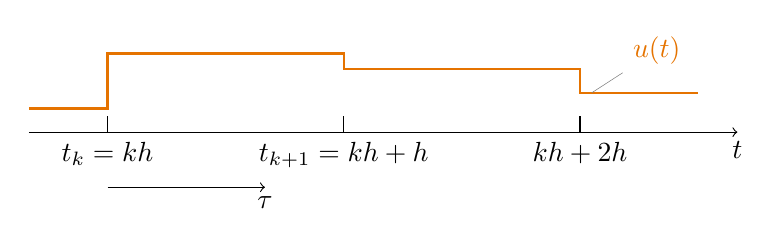
\begin{tikzpicture}
    \draw[->] (-3,0) -- (6,0) node[below] {$t$};
    \draw (-2, 0.2) -- ( -2, 0) node[below] {$t_k=kh$};
    \draw (1, 0.2) -- ( 1, 0) node[below] {$t_{k+1}=kh+h$};
    \draw (4, 0.2) -- ( 4, 0) node[below] {$kh+2h$};
    \draw[thick, orange!90!black] (-3,0.3) -- (-2, 0.3) -- (-2,1) -- (1, 1) -- (1,0.8) -- (4, 0.8) --(4, 0.5) --(5.5, 0.5) node[pos=0.1, coordinate, pin=30:{$u(t)$}] {} ; 
    \draw[->] (-2, -0.7) -- (0, -0.7) node[below] {$\tau$};
  \end{tikzpicture}
\end{center}

\pause

 \begin{align*}
  x(kh+h) &= \mathrm{e}^{Ah} x(kh) + \int_{0}^{h} \mathrm{e}^{As} B u(kh+h-s) ds\\
   &= \underbrace{\mathrm{e}^{Ah}}_{\Phi(h)} x(kh) + \underbrace{\left(\int_{0}^h \mathrm{e}^{As} B ds \right)}_{\Gamma(h)} u(kh)
\end{align*}
\end{frame}

\begin{frame}[label={sec:org8a9a709}]{Discretization - The matrix exponential}
\begin{center}
  \includegraphics[width=.7\linewidth]{../../figures/dubious.png}
\end{center}
\end{frame}

\begin{frame}[label={sec:orgf9cef9f}]{Discretization - The matrix exponential}
Square matrix \(A\). Scalar variable \(t\).
\[ \mathrm{e}^{At} = I + At + \frac{t^2}{2!}A^2 + \frac{t^3}{3!} A^3 + \cdots\]
Laplace transform
\[ \laplace{\mathrm{e}^{At}} = (sI - A)^{-1}\]
\end{frame}


\begin{frame}[label={sec:org03ba997}]{Discretization - example}
\small

 \begin{align*}
  x(kh+h) &= \mathrm{e}^{Ah} x(kh) + \int_{0}^{h} \mathrm{e}^{As} B u(kh+h-s) ds\\
   &= \underbrace{\mathrm{e}^{Ah}}_{\Phi(h)} x(kh) + \underbrace{\left(\int_{0}^h \mathrm{e}^{As} B ds \right)}_{\Gamma(h)} u(kh)
\end{align*}
\[ A = \begin{bmatrix} 0 & 0 & 0\\1 & 0 & 0\\0 & g & 0\end{bmatrix}, \quad A^2 = \begin{bmatrix} 0 & 0 & 0\\1 & 0 & 0\\0 & g & 0\end{bmatrix}\begin{bmatrix} 0 & 0 & 0\\1 & 0 & 0\\0 & g & 0\end{bmatrix}= \begin{bmatrix} 0 & 0 & 0\\0 & 0 & 0\\g & 0  & 0\end{bmatrix}, \quad A^3 = 0\]
So,
\begin{align*}
 \Phi(h) &= \mathrm{e}^{Ah} = I + Ah + A^2 h^2/2  + \cdots \\
\end{align*}

\pause

\begin{align*}
 \Phi(h) &= \begin{bmatrix} 1 & 0 & 0\\0 & 1 & 0\\0 & 0 & 1\end{bmatrix} + \begin{bmatrix} 0 & 0 & 0\\1 & 0 & 0\\0 & g & 0\end{bmatrix}h + \begin{bmatrix} 0 & 0 & 0\\0 & 0 & 0\\g & 0 & 0\end{bmatrix}\frac{h^ 2}{2}= \begin{bmatrix} 1 & 0 & 0\\h & 1 & 0\\\frac{h^2g}{2} & hg & 1\end{bmatrix}
 \end{align*}
\end{frame}

\begin{frame}[label={sec:org568062b}]{Discretization - example}
 \begin{align*}
  x(kh+h) &= \mathrm{e}^{Ah} x(kh) + \int_{0}^{h} \mathrm{e}^{As} B u(kh+h-s) ds\\
   &= \underbrace{\mathrm{e}^{Ah}}_{\Phi(h)} x(kh) + \underbrace{\left(\int_{0}^h \mathrm{e}^{As} B ds \right)}_{\Gamma(h)} u(kh)
\end{align*}
\[\mathrm{e}^{As}B &=  \begin{bmatrix} 1 & 0 & 0\\s & 1 & 0\\\frac{s^2g}{2} & sg & 1\end{bmatrix} \begin{bmatrix} \frac{1}{J}\\0\\0 \end{bmatrix} = \frac{1}{J} \begin{bmatrix} 1\\s\\\frac{gs^2}{2} \end{bmatrix}
  \]
\begin{align*}
\Gamma (h) &= \int_0^h \mathrm{e}^{As}B ds = \frac{1}{J} \int_0^h \begin{bmatrix} 1\\s\\\frac{gs^2}{2} \end{bmatrix}ds = \frac{1}{J}\begin{bmatrix} h\\ \frac{h^2}{2} \\ \frac{g h^3}{6} \end{bmatrix} 
\end{align*}
\end{frame}

\begin{frame}[label={sec:orgb414f0f}]{Discretization - example}
 \begin{align*}
  x(kh+h) &= \mathrm{e}^{Ah} x(kh) + \int_{0}^{h} \mathrm{e}^{As} B u(kh+h-s) ds\\
   &= \underbrace{\mathrm{e}^{Ah}}_{\Phi(h)} x(kh) + \underbrace{\left(\int_{0}^h \mathrm{e}^{As} B ds \right)}_{\Gamma(h)} u(kh)\\
   &= \begin{bmatrix} 1 & 0 & 0\\h & 1 & 0\\\frac{h^2g}{2} & hg & 1\end{bmatrix} x(kh) + \frac{1}{J} \begin{bmatrix} h\\ \frac{h^2}{2} \\ \frac{g h^3}{6} \end{bmatrix} u(kh)
\end{align*}
\end{frame}

\section{Stability}
\label{sec:org3e7227a}
\begin{frame}[label={sec:org68f96c3}]{Stability}
\end{frame}
\begin{frame}[label={sec:org6d21b1f}]{Eigenvalues and eigenvectors}
\alert{Definition} The eigenvalues \(\lambda_i  \in \mathbb{R}\) and eigenvectors \(v_i \in \mathbb{R}^n\) of a matrix \(\Phi \in \mathbb{R}^{n\times{}n}\) are the \(n\) pairs \((\lambda_i, v_i \neq 0 ), \; i=1,2,\ldots,n\) that satisfy
\[ \Phi v_i = \lambda_i v_i \]
\end{frame}

\begin{frame}[label={sec:orgd9a48bb}]{Stability}
The system
\begin{equation*}
x(k+1)=\Phi x(k), \ \ x(0)=x_0
\end{equation*}
is \alert{stable} if  \(\underset{t\to\infty}{\lim}x(kh)=0, \quad \forall\;  x_0\in\Bbb{R}^n\).

A necessary and sufficient requirement for stability is that \alert{all the eigenvalues of \(\Phi\) are inside the unit circle.}

The \alert{eigenvalues} of \(\Phi\) are the  \alert{poles} of the system.
\end{frame}

\section{State feedback}
\label{sec:org75d4b43}
\begin{frame}[label={sec:orgc029191}]{State feedback control}
\end{frame}
\begin{frame}[label={sec:orgb5b6f23}]{State feedback control}
Given
 \begin{equation}
 \begin{split}
  x(k+1) &= \Phi x(k) + \Gamma u(k)\\
  y(k) &= C x(k)
 \end{split}
 \label{eq:ssmodel}
\end{equation}
and measurements (or an estimate) of the state vector \(x(k)\). 

\alert{Linear state feedback} is the control law
\begin{equation*}
\begin{split}
 u(k) &= f\big((x(k), u_c(k)\big) = -\textcolor{morange}{l_1}x_1(k) - \textcolor{morange}{l_2}x_2(k) - \cdots - \textcolor{morange}{l_n} x_n(k) + \textcolor{mbluegreen}{l_0}u_c(k)\\
      &= -\textcolor{morange}{L}x(k) + \textcolor{mbluegreen}{l_0}u_c(k), 
\end{split}
\end{equation*}
where \[ \textcolor{morange}{L} = \bbm \textcolor{morange}{l_1} & \textcolor{morange}{l_2} & \cdots & \textcolor{morange}{l_n} \ebm. \]
Substituting this in the state-space model \eqref{eq:ssmodel} gives
 \begin{equation}
 \begin{split}
  x(k+1) &= \left(\Phi -\Gamma \textcolor{morange}{L} \right) x(k) + \textcolor{mbluegreen}{l_0}\Gamma u_c(k)\\
  y(k) &= C x(k)
 \end{split}
 \label{eq:closedloop}
\end{equation}
\end{frame}

\begin{frame}[label={sec:org1f6fa3e}]{Pole placement by state feedback}
Given (or choosing) a desired placement of the closed-loop poles \(p_1, p_2, \ldots, p_n\), being roots of the desired characteristic polynomial
\begin{equation}
a_c(z) = (z-p_1)(z-p_2)\cdots(z-p_n) = z^n + \alpha_1 z^{n-1} + \cdots \alpha_n.
\label{eq:desiredpoles}
\end{equation}

\pause

Linear state feedback gives the system
 \begin{equation}
 \begin{split}
  x(k+1) &= \left(\Phi -\Gamma \textcolor{morange}{L} \right) x(k) + \textcolor{mbluegreen}{l_0}\Gamma u_c(k)
 \end{split}
 \label{eq:closedloop}
\end{equation}
with characteristic polynomial
\begin{equation}
\det\left(zI - (\Phi - \Gamma \textcolor{morange}{L})\right) = z^n + \beta_1(\textcolor{morange}{l_1},\ldots,\textcolor{morange}{l_n}) z^{n-1} + \cdots \beta_n(\textcolor{morange}{l_1}, \ldots, \textcolor{morange}{l_n}).
\label{eq:poles}
\end{equation}

\pause

Set the coefficients of the desired characteristic polynomial \eqref{eq:desiredpoles} equal to the coefficients of \eqref{eq:poles} to obtain the system of equations
\begin{equation*}
\begin{split}
\beta_1(\textcolor{morange}{l_1}, \ldots, \textcolor{morange}{l_n}) &= \alpha_1\\
\beta_2(\textcolor{morange}{l_1}, \ldots, \textcolor{morange}{l_n}) &= \alpha_2\\
&\vdots\\
\beta_n(\textcolor{morange}{l_1}, \ldots, \textcolor{morange}{l_n}) &= \alpha_n
\end{split}
\label{eq:coeffs}
\end{equation*}
\end{frame}

\begin{frame}[label={sec:orgbacb088}]{Pole placement by state feedback}
The system of equations
\begin{equation*}
\begin{split}
\beta_1(\textcolor{morange}{l_1}, \ldots, \textcolor{morange}{l_n}) &= \alpha_1\\
\beta_2(\textcolor{morange}{l_1}, \ldots, \textcolor{morange}{l_n}) &= \alpha_2\\
&\vdots\\
\beta_n(\textcolor{morange}{l_1}, \ldots, \textcolor{morange}{l_n}) &= \alpha_n
\end{split}
\label{eq:coeffs}
\end{equation*}

is always linear in the parameters of the controller, hence
\begin{equation*}
M \textcolor{morange}{L}\transp = \alpha,
\end{equation*}
where \(\alpha\transp = \bbm \alpha_1 & \alpha_2 & \cdots & \alpha_n \ebm.\)
\end{frame}

\begin{frame}[label={sec:org86c6a79},fragile]{Pole placement by state feedback}
 Given a desired placement of the closed-loop poles \(p_1, p_2, \ldots, p_n\), being roots of the desired characteristic polynomial
\begin{equation*}
a_c(z) = (z-p_1)(z-p_2)\cdots(z-p_n) = z^n + \alpha_1 z^{n-1} + \cdots \alpha_n.
\label{eq:desiredpoles}
\end{equation*}
and closed-loop system
 \begin{equation*}
 \begin{split}
  x(k+1) &= \left(\Phi -\Gamma \textcolor{morange}{L} \right) x(k) + \textcolor{mbluegreen}{l_0}\Gamma u_c(k)\\
  y(k) &= C x(k)
 \end{split}
 \label{eq:closedloop}
\end{equation*}

The Matlab (\emph{control systems toolbox}) has methods for computing the gain vector \(L\)

\begin{enumerate}
\item \alert{Ackerman's method} 
\begin{verbatim}
L = acker(Phi, Gamma, pd)
\end{verbatim}
\item \alert{Numerically more stable method} 
\begin{verbatim}
L = place(Phi, Gamma, pd)
\end{verbatim}
\end{enumerate}
\end{frame}

\begin{frame}[label={sec:org41f1c99}]{The reference input gain \(l_0\)}
The closed-loop state space system
\begin{equation*}
\begin{split}
 x(k+1) &= \underbrace{\left(\Phi -\Gamma \textcolor{morange}{L} \right)}_{\Phi_c} x(k) + \textcolor{mbluegreen}{l_0}\Gamma u_c(k)\\
 y(k) &= C x(k)
\end{split}
\end{equation*}
with constant reference signal \(u_c(k) = u_{c,f}\) has the steady-state solution (\(x(k+1)=x(k)\))
\pause
\[ x_f =  \textcolor{mbluegreen}{l_0} (I - \Phi_c)^{-1}\Gamma u_{c,f}\]
\[ y_f = Cx_f = \textcolor{mbluegreen}{l_0} C(I - \Phi_c)^{-1}\Gamma u_{c,f}.\]
We want \(y_f =  u_{c,f}\),
\[ \Rightarrow \qquad \textcolor{mbluegreen}{l_0} = \frac{1}{C(I-\Phi_c)^{-1}\Gamma}\]
\end{frame}
\end{document}